\documentclass[../main.tex]{subfiles}
\thispagestyle{header-pages}
\begin{document}

\newcommand{\requirement}[5]{
    \bgroup{}
    \def\arraystretch{1.25}
    \begin{center}
        \begin{tabular}{|l|p{9cm}| }
            \hline
            \multicolumn{2}{|c|}{\textbf{ID: Req-#1}} \\
            \hline
            \textbf{Nome} & #2 \\
            \hline
            \textbf{Priorità} & #3 \\
            \hline
            \textbf{Versione} & #4 \\
            \hline
            \textbf{Note} & #5 \\
            \hline
        \end{tabular}
    \end{center}
    \egroup{}
}

\subsection{Analisi del dominio}
È stato richiesto di creare sistema che abbia due server e che questi due siano ridondanti, i due server non devono avere servizzi replicati, inoltre, deve essere presente anche un sistema dfs su un altro server per FTP con ridondanza. Devono anche esserci 3 pc per testare tutto il sistema tirato in piedi. Deve essere anche peresente un sistema di backup per le modifiche giornaliere. 


Tutto il sistema verrà creato su Server Win 2019


\subsection{Analisi dei mezzi}

    \subsubsection{Software}
\begin{itemize}
    \item VirtualBox 6.1
    \item Windows Server 2019
    \item Windows 10 21H1 versione English
    \item Windows 10 20H2 versione Italiana

\end{itemize}



\subsubsection{Hardware}
\begin{itemize}
    \item PC scolastic
    \item Server sv-104-qnap2


\end{itemize}

\pagebreak{}
\thispagestyle{header-pages}

\subsection{Analisi e specifica dei requisiti}


\requirement{01}
    {Avere due server}
    {1}
    {1.1}
    {Sistema operativo Windos 2019}

\requirement{02}
    {Deve essere presente il sistema ADDS}
    {1}
    {1.1}
    {}

\requirement{03}
    {Deve essere presente il sistema DNS}
    {1}
    {1.1}
    {}
    
\requirement{04}
    {Deve essere presente il sistema GPO}
    {1}
    {1.1}
    {}

\requirement{05}
    {Deve essere presente il DHCP }
    {1}
    {1.1}
    {}
    
\pagebreak{}
\thispagestyle{header-pages}
\requirement{06}
    {Deve essere presente un File Server }
    {1}
    {1.1}
    {}
    

\requirement{07}
    {Tutti i servizzi ridondanti}
    {1}
    {1.1}
    {}

\requirement{08}
    {Gestire le cartelle condivise}
    {1}
    {1.1}
    {Si devono poter gestire da qualssiasi pc}
 
\requirement{09}
    {Server con base di dati condivisa}
    {1}
    {1.1}
    {}

\requirement{10}
    {10 Utenti attivi}
    {1}
    {1.1}
    {Direttore,Vice, Segretaria, sistemista e 6 impiegati}
    
\pagebreak{}
\thispagestyle{header-pages}

\requirement{11}
    {Cartelle condivise con GPO}
    {1}
    {1.1}
    {}

\requirement{12}
    {Salvare ogni giorno la base di dati}
    {2}
    {1.1}
    {}

\requirement{13}
    {3 VM Win 10 per test e soluione}
    {2}
    {1.1}
    {}
    
\requirement{14}
    {Manuale Utente}
    {2}
    {1.1}
    {}



\subsection{Use case}

I casi d’uso rappresentano l’interazione tra i vari attori e le
funzionalità del prodotto.

\pagebreak{}
\thispagestyle{header-pages}
\subsection{Pianificazione}

Per la pianificazione alleghiamo il Gantt preventivo che ho stabilito:
 \begin{figure}[h]
    \centering
    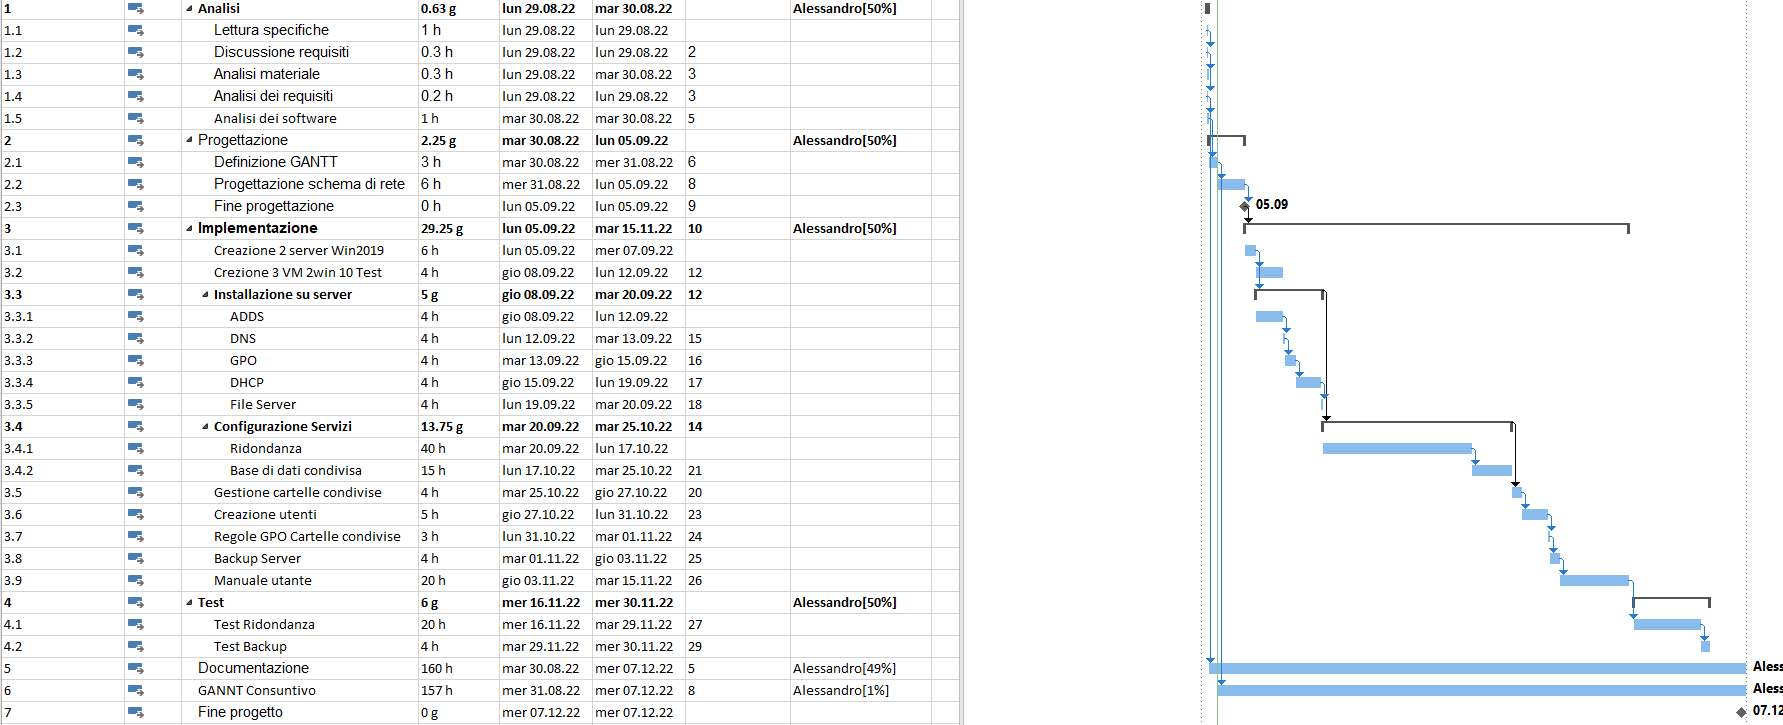
\includegraphics[width=1\textwidth]{Images/GANTT_Preventivo_Completo.jpg}
    \caption{Gantt preventivo}
\end{figure}

\end{document}